\documentclass[twoside]{book}

% Packages required by doxygen
\usepackage{fixltx2e}
\usepackage{calc}
\usepackage{doxygen}
\usepackage[export]{adjustbox} % also loads graphicx
\usepackage{graphicx}
\usepackage[utf8]{inputenc}
\usepackage{makeidx}
\usepackage{multicol}
\usepackage{multirow}
\PassOptionsToPackage{warn}{textcomp}
\usepackage{textcomp}
\usepackage[nointegrals]{wasysym}
\usepackage[table]{xcolor}

% Font selection
\usepackage[T1]{fontenc}
\usepackage[scaled=.90]{helvet}
\usepackage{courier}
\usepackage{amssymb}
\usepackage{sectsty}
\renewcommand{\familydefault}{\sfdefault}
\allsectionsfont{%
  \fontseries{bc}\selectfont%
  \color{darkgray}%
}
\renewcommand{\DoxyLabelFont}{%
  \fontseries{bc}\selectfont%
  \color{darkgray}%
}
\newcommand{\+}{\discretionary{\mbox{\scriptsize$\hookleftarrow$}}{}{}}

% Page & text layout
\usepackage{geometry}
\geometry{%
  a4paper,%
  top=2.5cm,%
  bottom=2.5cm,%
  left=2.5cm,%
  right=2.5cm%
}
\tolerance=750
\hfuzz=15pt
\hbadness=750
\setlength{\emergencystretch}{15pt}
\setlength{\parindent}{0cm}
\setlength{\parskip}{0.2cm}
\makeatletter
\renewcommand{\paragraph}{%
  \@startsection{paragraph}{4}{0ex}{-1.0ex}{1.0ex}{%
    \normalfont\normalsize\bfseries\SS@parafont%
  }%
}
\renewcommand{\subparagraph}{%
  \@startsection{subparagraph}{5}{0ex}{-1.0ex}{1.0ex}{%
    \normalfont\normalsize\bfseries\SS@subparafont%
  }%
}
\makeatother

% Headers & footers
\usepackage{fancyhdr}
\pagestyle{fancyplain}
\fancyhead[LE]{\fancyplain{}{\bfseries\thepage}}
\fancyhead[CE]{\fancyplain{}{}}
\fancyhead[RE]{\fancyplain{}{\bfseries\leftmark}}
\fancyhead[LO]{\fancyplain{}{\bfseries\rightmark}}
\fancyhead[CO]{\fancyplain{}{}}
\fancyhead[RO]{\fancyplain{}{\bfseries\thepage}}
\fancyfoot[LE]{\fancyplain{}{}}
\fancyfoot[CE]{\fancyplain{}{}}
\fancyfoot[RE]{\fancyplain{}{\bfseries\scriptsize Generated on Thu Mar 12 2015 19\+:13\+:56 for M\+D\+L by Doxygen }}
\fancyfoot[LO]{\fancyplain{}{\bfseries\scriptsize Generated on Thu Mar 12 2015 19\+:13\+:56 for M\+D\+L by Doxygen }}
\fancyfoot[CO]{\fancyplain{}{}}
\fancyfoot[RO]{\fancyplain{}{}}
\renewcommand{\footrulewidth}{0.4pt}
\renewcommand{\chaptermark}[1]{%
  \markboth{#1}{}%
}
\renewcommand{\sectionmark}[1]{%
  \markright{\thesection\ #1}%
}

% Indices & bibliography
\usepackage{natbib}
\usepackage[titles]{tocloft}
\setcounter{tocdepth}{3}
\setcounter{secnumdepth}{5}
\makeindex

% Hyperlinks (required, but should be loaded last)
\usepackage{ifpdf}
\ifpdf
  \usepackage[pdftex,pagebackref=true]{hyperref}
\else
  \usepackage[ps2pdf,pagebackref=true]{hyperref}
\fi
\hypersetup{%
  colorlinks=true,%
  linkcolor=blue,%
  citecolor=blue,%
  unicode%
}

% Custom commands
\newcommand{\clearemptydoublepage}{%
  \newpage{\pagestyle{empty}\cleardoublepage}%
}


%===== C O N T E N T S =====

\begin{document}

% Titlepage & ToC
\hypersetup{pageanchor=false,
             bookmarks=true,
             bookmarksnumbered=true,
             pdfencoding=unicode
            }
\pagenumbering{roman}
\begin{titlepage}
\vspace*{7cm}
\begin{center}%
{\Large M\+D\+L }\\
\vspace*{1cm}
{\large Generated by Doxygen 1.8.9.1}\\
\vspace*{0.5cm}
{\small Thu Mar 12 2015 19:13:56}\\
\end{center}
\end{titlepage}
\clearemptydoublepage
\tableofcontents
\clearemptydoublepage
\pagenumbering{arabic}
\hypersetup{pageanchor=true}

%--- Begin generated contents ---
\chapter{Namespace Index}
\section{Packages}
Here are the packages with brief descriptions (if available)\+:\begin{DoxyCompactList}
\item\contentsline{section}{\hyperlink{namespace_base_de_donnees}{Base\+De\+Donnees} }{\pageref{namespace_base_de_donnees}}{}
\item\contentsline{section}{\hyperlink{namespace_maison_des_ligues}{Maison\+Des\+Ligues} }{\pageref{namespace_maison_des_ligues}}{}
\end{DoxyCompactList}

\chapter{Hierarchical Index}
\section{Class Hierarchy}
This inheritance list is sorted roughly, but not completely, alphabetically\+:\begin{DoxyCompactList}
\item \contentsline{section}{Base\+De\+Donnees.\+Bdd}{\pageref{class_base_de_donnees_1_1_bdd}}{}
\item Form\begin{DoxyCompactList}
\item \contentsline{section}{Maison\+Des\+Ligues.\+Frm\+Login}{\pageref{class_maison_des_ligues_1_1_frm_login}}{}
\item \contentsline{section}{Maison\+Des\+Ligues.\+Frm\+Principale}{\pageref{class_maison_des_ligues_1_1_frm_principale}}{}
\end{DoxyCompactList}
\end{DoxyCompactList}

\chapter{Class Index}
\section{Class List}
Here are the classes, structs, unions and interfaces with brief descriptions\+:\begin{DoxyCompactList}
\item\contentsline{section}{\hyperlink{class_base_de_donnees_1_1_bdd}{Base\+De\+Donnees.\+Bdd} }{\pageref{class_base_de_donnees_1_1_bdd}}{}
\item\contentsline{section}{\hyperlink{class_maison_des_ligues_1_1_frm_login}{Maison\+Des\+Ligues.\+Frm\+Login} }{\pageref{class_maison_des_ligues_1_1_frm_login}}{}
\item\contentsline{section}{\hyperlink{class_maison_des_ligues_1_1_frm_principale}{Maison\+Des\+Ligues.\+Frm\+Principale} }{\pageref{class_maison_des_ligues_1_1_frm_principale}}{}
\end{DoxyCompactList}

\chapter{Namespace Documentation}
\hypertarget{namespace_base_de_donnees}{}\section{Package Base\+De\+Donnees}
\label{namespace_base_de_donnees}\index{Base\+De\+Donnees@{Base\+De\+Donnees}}
\subsection*{Classes}
\begin{DoxyCompactItemize}
\item 
class \hyperlink{class_base_de_donnees_1_1_bdd}{Bdd}
\end{DoxyCompactItemize}

\hypertarget{namespace_maison_des_ligues}{}\section{Package Maison\+Des\+Ligues}
\label{namespace_maison_des_ligues}\index{Maison\+Des\+Ligues@{Maison\+Des\+Ligues}}
\subsection*{Classes}
\begin{DoxyCompactItemize}
\item 
class \hyperlink{class_maison_des_ligues_1_1_frm_login}{Frm\+Login}
\item 
class \hyperlink{class_maison_des_ligues_1_1_frm_principale}{Frm\+Principale}
\item 
class {\bfseries Program}
\item 
class {\bfseries Utilitaire}
\end{DoxyCompactItemize}

\chapter{Class Documentation}
\hypertarget{class_base_de_donnees_1_1_bdd}{}\section{Base\+De\+Donnees.\+Bdd Class Reference}
\label{class_base_de_donnees_1_1_bdd}\index{Base\+De\+Donnees.\+Bdd@{Base\+De\+Donnees.\+Bdd}}
\subsection*{Public Member Functions}
\begin{DoxyCompactItemize}
\item 
\hyperlink{class_base_de_donnees_1_1_bdd_ab7425636f7b6865411160424455ddacf}{Bdd} (String Un\+Login, String Un\+Pwd)
\begin{DoxyCompactList}\small\item\em constructeur de la connexion \end{DoxyCompactList}\item 
void \hyperlink{class_base_de_donnees_1_1_bdd_aa75a70827f654db3f17b9451975446bb}{Fermer\+Connexion} ()
\begin{DoxyCompactList}\small\item\em Méthode permettant de fermer la connexion \end{DoxyCompactList}\item 
Data\+Table \hyperlink{class_base_de_donnees_1_1_bdd_a1f5203fd6378328a9545b47b7dd6bd97}{Obtenir\+Donnes\+Oracle} (String Une\+Table\+Ou\+Vue)
\begin{DoxyCompactList}\small\item\em permet de récupérer le contenu d\textquotesingle{}une table ou d\textquotesingle{}une vue. \end{DoxyCompactList}\item 
void \hyperlink{class_base_de_donnees_1_1_bdd_ac60e11f0e915babf2a78d168bf7a744e}{Inscrire\+Benevole} (String p\+Nom, String p\+Prenom, String p\+Adresse1, String p\+Adresse2, String p\+Cp, String p\+Ville, String p\+Tel, String p\+Mail, Date\+Time p\+Date\+Naissance, Int64?p\+Numero\+Licence, Collection$<$ Int16 $>$ p\+Date\+Benevolat)
\begin{DoxyCompactList}\small\item\em procédure qui va se charger d\textquotesingle{}invoquer la procédure stockée qui ira inscrire un participant de type bénévole \end{DoxyCompactList}\item 
void \hyperlink{class_base_de_donnees_1_1_bdd_a0974d13870c2fdb8484d5f7b2d283f1a}{Inscrire\+Licencie} (String p\+Nom, String p\+Prenom, String p\+Adresse1, String p\+Adresse2, String p\+Cp, String p\+Ville, String p\+Tel, String p\+Mail, Int64 p\+Numero\+Licence, Int32 p\+Qualite, Int16 p\+Id\+Atelier, Int64 p\+Num\+Cheque, Int64 p\+Montant)
\begin{DoxyCompactList}\small\item\em Procedure d\textquotesingle{}inscription d\textquotesingle{}un licencie sans nuite et sans restauration \end{DoxyCompactList}\item 
void \hyperlink{class_base_de_donnees_1_1_bdd_af80619478c0d65bc2044a6add59195c6}{Inscrire\+Licencie} (String p\+Nom, String p\+Prenom, String p\+Adresse1, String p\+Adresse2, String p\+Cp, String p\+Ville, String p\+Tel, String p\+Mail, Int64 p\+Numero\+Licence, Int32 p\+Qualite, Int16 p\+Id\+Atelier, Collection$<$ string $>$ p\+Les\+Categories, Collection$<$ string $>$ p\+Les\+Hotels, Collection$<$ Int16 $>$ p\+Les\+Nuits, Int64 p\+Num\+Cheque, Int64 p\+Montant)
\begin{DoxyCompactList}\small\item\em Procedure d\textquotesingle{}inscription d\textquotesingle{}un licencie avec les nuites mais sans la restauration \end{DoxyCompactList}\item 
void \hyperlink{class_base_de_donnees_1_1_bdd_a4ba18acfc209c903383908ad94ee83b9}{Inscrire\+Licencie} (String p\+Nom, String p\+Prenom, String p\+Adresse1, String p\+Adresse2, String p\+Cp, String p\+Ville, String p\+Tel, String p\+Mail, Int64 p\+Numero\+Licence, Int32 p\+Qualite, Int16 p\+Id\+Atelier, Collection$<$ string $>$ p\+Les\+Categories, Collection$<$ string $>$ p\+Les\+Hotels, Collection$<$ Int16 $>$ p\+Les\+Nuits, Collection$<$ String $>$ p\+Restauration, Int64 p\+Num\+Cheque, Int64 p\+Montant)
\begin{DoxyCompactList}\small\item\em Procedure d\textquotesingle{}inscription d\textquotesingle{}un licencie avec les nuites et les restaurations \end{DoxyCompactList}\item 
void \hyperlink{class_base_de_donnees_1_1_bdd_abfbf2eb771a5e60ef361d5d9fc00304f}{Inscrire\+Intervenant} (String p\+Nom, String p\+Prenom, String p\+Adresse1, String p\+Adresse2, String p\+Cp, String p\+Ville, String p\+Tel, String p\+Mail, Int16 p\+Id\+Atelier, String p\+Id\+Statut)
\begin{DoxyCompactList}\small\item\em Procédure publique qui va appeler la procédure stockée permettant d\textquotesingle{}inscrire un nouvel intervenant sans nuité \end{DoxyCompactList}\item 
void \hyperlink{class_base_de_donnees_1_1_bdd_a2ecae01b408afab3f2457286b9bc6cc7}{Inscrire\+Intervenant} (String p\+Nom, String p\+Prenom, String p\+Adresse1, String p\+Adresse2, String p\+Cp, String p\+Ville, String p\+Tel, String p\+Mail, Int16 p\+Id\+Atelier, String p\+Id\+Statut, Collection$<$ string $>$ p\+Les\+Categories, Collection$<$ string $>$ p\+Les\+Hotels, Collection$<$ Int16 $>$ p\+Les\+Nuits)
\begin{DoxyCompactList}\small\item\em Procédure publique qui va appeler la procédure stockée permettant d\textquotesingle{}inscrire un nouvel intervenant qui aura des nuités \end{DoxyCompactList}\item 
Dictionary$<$ Int16, String $>$ \hyperlink{class_base_de_donnees_1_1_bdd_af48b871d33fdfd845de9d4012109d00f}{Obtenir\+Dates\+Nuites} ()
\begin{DoxyCompactList}\small\item\em fonction permettant de construire un dictionnaire dont l\textquotesingle{}id est l\textquotesingle{}id d\textquotesingle{}une nuité et le contenu une date sous la la forme \+: lundi 7 janvier 2013 /// \end{DoxyCompactList}\item 
void \hyperlink{class_base_de_donnees_1_1_bdd_a1e3e6db107c1b88da6e57d8e008e6df4}{Ajout\+Theme} (Int16 p\+Id\+Atelier, String p\+Libelle\+Theme)
\begin{DoxyCompactList}\small\item\em Méthode qui permet d\textquotesingle{}ajouter un theme dans un atelier \end{DoxyCompactList}\item 
void \hyperlink{class_base_de_donnees_1_1_bdd_a94b0407a64c613c1b1ed1f1d57741a5e}{Ajout\+Vacation} (Int16 p\+Id\+Atelier, Date\+Time p\+Heure\+Dbt, Date\+Time p\+Heure\+Fin)
\begin{DoxyCompactList}\small\item\em methode public qui permet de faire appel a la procedure stockée ajoutvacation du package pckatelier pour ajouter une vacation a un atelier \end{DoxyCompactList}\item 
void \hyperlink{class_base_de_donnees_1_1_bdd_ad41e17409a13d72fdcc4238804ad7c54}{Ajout\+Atelier} (String p\+Libelle\+Atelier, Int32 p\+Nb\+Places\+Maxi, Collection$<$ C\+Theme $>$ p\+Les\+Themes, Collection$<$ C\+Vacation $>$ p\+Les\+Vacation)
\begin{DoxyCompactList}\small\item\em méthode qui permet de faire appel a la procedure stockée creervacation du package pckatelier pour creer un atelier \end{DoxyCompactList}\item 
Collection$<$ C\+Vacation $>$ \hyperlink{class_base_de_donnees_1_1_bdd_a4c78979c04e05eb1c33d903d73aa737e}{Get\+Vacations} (int p\+Id\+Atelier)
\begin{DoxyCompactList}\small\item\em fonction qui récupére les vacations d\textquotesingle{}un atelier et les retournes sous forme de composant vacation \end{DoxyCompactList}\item 
void \hyperlink{class_base_de_donnees_1_1_bdd_a7d6d9ec30677d955898387f6504a73d2}{Update\+Vacation} (Collection$<$ C\+Vacation $>$p\+Les\+Vacation, Int32 p\+Id\+Atelier)
\begin{DoxyCompactList}\small\item\em methode qui permet de mettre a jour les vacations d\textquotesingle{}un atelier \end{DoxyCompactList}\end{DoxyCompactItemize}


\subsection{Constructor \& Destructor Documentation}
\hypertarget{class_base_de_donnees_1_1_bdd_ab7425636f7b6865411160424455ddacf}{}\index{Base\+De\+Donnees\+::\+Bdd@{Base\+De\+Donnees\+::\+Bdd}!Bdd@{Bdd}}
\index{Bdd@{Bdd}!Base\+De\+Donnees\+::\+Bdd@{Base\+De\+Donnees\+::\+Bdd}}
\subsubsection[{Bdd}]{\setlength{\rightskip}{0pt plus 5cm}Base\+De\+Donnees.\+Bdd.\+Bdd (
\begin{DoxyParamCaption}
\item[{String}]{Un\+Login, }
\item[{String}]{Un\+Pwd}
\end{DoxyParamCaption}
)}\label{class_base_de_donnees_1_1_bdd_ab7425636f7b6865411160424455ddacf}


constructeur de la connexion 


\begin{DoxyParams}{Parameters}
{\em Un\+Login} & login utilisateur\\
\hline
{\em Un\+Pwd} & mot de passe utilisateur\\
\hline
\end{DoxyParams}
on commence par récupérer dans Cn\+String les informations contenues dans le fichier app.\+config pour la connection\+String de nom Str\+Conn\+Mdl 

on va remplacer dans la chaine de connexion les paramètres par le login et le pwd saisis dans les zones de texte. Pour ça on va utiliser la méthode Format de la classe String. /// 

\subsection{Member Function Documentation}
\hypertarget{class_base_de_donnees_1_1_bdd_ad41e17409a13d72fdcc4238804ad7c54}{}\index{Base\+De\+Donnees\+::\+Bdd@{Base\+De\+Donnees\+::\+Bdd}!Ajout\+Atelier@{Ajout\+Atelier}}
\index{Ajout\+Atelier@{Ajout\+Atelier}!Base\+De\+Donnees\+::\+Bdd@{Base\+De\+Donnees\+::\+Bdd}}
\subsubsection[{Ajout\+Atelier}]{\setlength{\rightskip}{0pt plus 5cm}void Base\+De\+Donnees.\+Bdd.\+Ajout\+Atelier (
\begin{DoxyParamCaption}
\item[{String}]{p\+Libelle\+Atelier, }
\item[{Int32}]{p\+Nb\+Places\+Maxi, }
\item[{Collection$<$ C\+Theme $>$}]{p\+Les\+Themes, }
\item[{Collection$<$ C\+Vacation $>$}]{p\+Les\+Vacation}
\end{DoxyParamCaption}
)}\label{class_base_de_donnees_1_1_bdd_ad41e17409a13d72fdcc4238804ad7c54}


méthode qui permet de faire appel a la procedure stockée creervacation du package pckatelier pour creer un atelier 


\begin{DoxyParams}{Parameters}
{\em p\+Libelle\+Atelier} & \\
\hline
{\em p\+Nb\+Places\+Maxi} & \\
\hline
{\em p\+Les\+Themes} & \\
\hline
{\em p\+Les\+Vacations} & \\
\hline
\end{DoxyParams}
\hypertarget{class_base_de_donnees_1_1_bdd_a1e3e6db107c1b88da6e57d8e008e6df4}{}\index{Base\+De\+Donnees\+::\+Bdd@{Base\+De\+Donnees\+::\+Bdd}!Ajout\+Theme@{Ajout\+Theme}}
\index{Ajout\+Theme@{Ajout\+Theme}!Base\+De\+Donnees\+::\+Bdd@{Base\+De\+Donnees\+::\+Bdd}}
\subsubsection[{Ajout\+Theme}]{\setlength{\rightskip}{0pt plus 5cm}void Base\+De\+Donnees.\+Bdd.\+Ajout\+Theme (
\begin{DoxyParamCaption}
\item[{Int16}]{p\+Id\+Atelier, }
\item[{String}]{p\+Libelle\+Theme}
\end{DoxyParamCaption}
)}\label{class_base_de_donnees_1_1_bdd_a1e3e6db107c1b88da6e57d8e008e6df4}


Méthode qui permet d\textquotesingle{}ajouter un theme dans un atelier 


\begin{DoxyParams}{Parameters}
{\em p\+Id\+Atelier} & \\
\hline
{\em p\+Libelle\+Theme} & \\
\hline
\end{DoxyParams}
\hypertarget{class_base_de_donnees_1_1_bdd_a94b0407a64c613c1b1ed1f1d57741a5e}{}\index{Base\+De\+Donnees\+::\+Bdd@{Base\+De\+Donnees\+::\+Bdd}!Ajout\+Vacation@{Ajout\+Vacation}}
\index{Ajout\+Vacation@{Ajout\+Vacation}!Base\+De\+Donnees\+::\+Bdd@{Base\+De\+Donnees\+::\+Bdd}}
\subsubsection[{Ajout\+Vacation}]{\setlength{\rightskip}{0pt plus 5cm}void Base\+De\+Donnees.\+Bdd.\+Ajout\+Vacation (
\begin{DoxyParamCaption}
\item[{Int16}]{p\+Id\+Atelier, }
\item[{Date\+Time}]{p\+Heure\+Dbt, }
\item[{Date\+Time}]{p\+Heure\+Fin}
\end{DoxyParamCaption}
)}\label{class_base_de_donnees_1_1_bdd_a94b0407a64c613c1b1ed1f1d57741a5e}


methode public qui permet de faire appel a la procedure stockée ajoutvacation du package pckatelier pour ajouter une vacation a un atelier 


\begin{DoxyParams}{Parameters}
{\em p\+Id\+Atelier} & Id de l\textquotesingle{}atelier passa au quel on ajoute une vacation\\
\hline
{\em p\+Heure\+Dbt} & date et heure du debut de la vacation\\
\hline
{\em p\+Heure\+Fin} & date et heure de la fin de la vacation\\
\hline
\end{DoxyParams}
\hypertarget{class_base_de_donnees_1_1_bdd_aa75a70827f654db3f17b9451975446bb}{}\index{Base\+De\+Donnees\+::\+Bdd@{Base\+De\+Donnees\+::\+Bdd}!Fermer\+Connexion@{Fermer\+Connexion}}
\index{Fermer\+Connexion@{Fermer\+Connexion}!Base\+De\+Donnees\+::\+Bdd@{Base\+De\+Donnees\+::\+Bdd}}
\subsubsection[{Fermer\+Connexion}]{\setlength{\rightskip}{0pt plus 5cm}void Base\+De\+Donnees.\+Bdd.\+Fermer\+Connexion (
\begin{DoxyParamCaption}
{}
\end{DoxyParamCaption}
)}\label{class_base_de_donnees_1_1_bdd_aa75a70827f654db3f17b9451975446bb}


Méthode permettant de fermer la connexion 

\hypertarget{class_base_de_donnees_1_1_bdd_a4c78979c04e05eb1c33d903d73aa737e}{}\index{Base\+De\+Donnees\+::\+Bdd@{Base\+De\+Donnees\+::\+Bdd}!Get\+Vacations@{Get\+Vacations}}
\index{Get\+Vacations@{Get\+Vacations}!Base\+De\+Donnees\+::\+Bdd@{Base\+De\+Donnees\+::\+Bdd}}
\subsubsection[{Get\+Vacations}]{\setlength{\rightskip}{0pt plus 5cm}Collection$<$C\+Vacation$>$ Base\+De\+Donnees.\+Bdd.\+Get\+Vacations (
\begin{DoxyParamCaption}
\item[{int}]{p\+Id\+Atelier}
\end{DoxyParamCaption}
)}\label{class_base_de_donnees_1_1_bdd_a4c78979c04e05eb1c33d903d73aa737e}


fonction qui récupére les vacations d\textquotesingle{}un atelier et les retournes sous forme de composant vacation 


\begin{DoxyParams}{Parameters}
{\em p\+Id\+Atelier} & \\
\hline
\end{DoxyParams}
\begin{DoxyReturn}{Returns}

\end{DoxyReturn}
\hypertarget{class_base_de_donnees_1_1_bdd_ac60e11f0e915babf2a78d168bf7a744e}{}\index{Base\+De\+Donnees\+::\+Bdd@{Base\+De\+Donnees\+::\+Bdd}!Inscrire\+Benevole@{Inscrire\+Benevole}}
\index{Inscrire\+Benevole@{Inscrire\+Benevole}!Base\+De\+Donnees\+::\+Bdd@{Base\+De\+Donnees\+::\+Bdd}}
\subsubsection[{Inscrire\+Benevole}]{\setlength{\rightskip}{0pt plus 5cm}void Base\+De\+Donnees.\+Bdd.\+Inscrire\+Benevole (
\begin{DoxyParamCaption}
\item[{String}]{p\+Nom, }
\item[{String}]{p\+Prenom, }
\item[{String}]{p\+Adresse1, }
\item[{String}]{p\+Adresse2, }
\item[{String}]{p\+Cp, }
\item[{String}]{p\+Ville, }
\item[{String}]{p\+Tel, }
\item[{String}]{p\+Mail, }
\item[{Date\+Time}]{p\+Date\+Naissance, }
\item[{Int64?}]{p\+Numero\+Licence, }
\item[{Collection$<$ Int16 $>$}]{p\+Date\+Benevolat}
\end{DoxyParamCaption}
)}\label{class_base_de_donnees_1_1_bdd_ac60e11f0e915babf2a78d168bf7a744e}


procédure qui va se charger d\textquotesingle{}invoquer la procédure stockée qui ira inscrire un participant de type bénévole 


\begin{DoxyParams}{Parameters}
{\em Cmd} & nom de l\textquotesingle{}objet command concerné par les paramètres\\
\hline
{\em p\+Nom} & nom du participant\\
\hline
{\em p\+Prenom} & prénom du participant\\
\hline
{\em p\+Adresse1} & adresse1 du participant\\
\hline
{\em p\+Adresse2} & adresse2 du participant\\
\hline
{\em p\+Cp} & cp du participant\\
\hline
{\em p\+Ville} & ville du participant\\
\hline
{\em p\+Tel} & téléphone du participant\\
\hline
{\em p\+Mail} & mail du participant\\
\hline
{\em p\+Date\+Naissance} & mail du bénévole\\
\hline
{\em p\+Numero\+Licence} & numéro de licence du bénévole ou null\\
\hline
{\em p\+Date\+Benevolat} & collection des id des dates où le bénévole sera présent\\
\hline
\end{DoxyParams}
\hypertarget{class_base_de_donnees_1_1_bdd_abfbf2eb771a5e60ef361d5d9fc00304f}{}\index{Base\+De\+Donnees\+::\+Bdd@{Base\+De\+Donnees\+::\+Bdd}!Inscrire\+Intervenant@{Inscrire\+Intervenant}}
\index{Inscrire\+Intervenant@{Inscrire\+Intervenant}!Base\+De\+Donnees\+::\+Bdd@{Base\+De\+Donnees\+::\+Bdd}}
\subsubsection[{Inscrire\+Intervenant}]{\setlength{\rightskip}{0pt plus 5cm}void Base\+De\+Donnees.\+Bdd.\+Inscrire\+Intervenant (
\begin{DoxyParamCaption}
\item[{String}]{p\+Nom, }
\item[{String}]{p\+Prenom, }
\item[{String}]{p\+Adresse1, }
\item[{String}]{p\+Adresse2, }
\item[{String}]{p\+Cp, }
\item[{String}]{p\+Ville, }
\item[{String}]{p\+Tel, }
\item[{String}]{p\+Mail, }
\item[{Int16}]{p\+Id\+Atelier, }
\item[{String}]{p\+Id\+Statut}
\end{DoxyParamCaption}
)}\label{class_base_de_donnees_1_1_bdd_abfbf2eb771a5e60ef361d5d9fc00304f}


Procédure publique qui va appeler la procédure stockée permettant d\textquotesingle{}inscrire un nouvel intervenant sans nuité 


\begin{DoxyParams}{Parameters}
{\em Cmd} & nom de l\textquotesingle{}objet command concerné par les paramètres\\
\hline
{\em p\+Nom} & nom du participant\\
\hline
{\em p\+Prenom} & prénom du participant\\
\hline
{\em p\+Adresse1} & adresse1 du participant\\
\hline
{\em p\+Adresse2} & adresse2 du participant\\
\hline
{\em p\+Cp} & cp du participant\\
\hline
{\em p\+Ville} & ville du participant\\
\hline
{\em p\+Tel} & téléphone du participant\\
\hline
{\em p\+Mail} & mail du participant\\
\hline
{\em p\+Id\+Atelier} & Id de l\textquotesingle{}atelier où interviendra l\textquotesingle{}intervenant\\
\hline
{\em p\+Id\+Statut} & statut de l\textquotesingle{}intervenant pour l\textquotesingle{}atelier \+: animateur ou intervenant\\
\hline
\end{DoxyParams}
procédure qui va créer \+: 1-\/ un enregistrement dans la table participant 2-\/ un enregistrement dans la table intervenant en cas d\textquotesingle{}erreur Oracle, appel à la méthode Get\+Message\+Oracle dont le rôle est d\textquotesingle{}extraire uniquement le message renvoyé par une procédure ou un trigger Oracle \hypertarget{class_base_de_donnees_1_1_bdd_a2ecae01b408afab3f2457286b9bc6cc7}{}\index{Base\+De\+Donnees\+::\+Bdd@{Base\+De\+Donnees\+::\+Bdd}!Inscrire\+Intervenant@{Inscrire\+Intervenant}}
\index{Inscrire\+Intervenant@{Inscrire\+Intervenant}!Base\+De\+Donnees\+::\+Bdd@{Base\+De\+Donnees\+::\+Bdd}}
\subsubsection[{Inscrire\+Intervenant}]{\setlength{\rightskip}{0pt plus 5cm}void Base\+De\+Donnees.\+Bdd.\+Inscrire\+Intervenant (
\begin{DoxyParamCaption}
\item[{String}]{p\+Nom, }
\item[{String}]{p\+Prenom, }
\item[{String}]{p\+Adresse1, }
\item[{String}]{p\+Adresse2, }
\item[{String}]{p\+Cp, }
\item[{String}]{p\+Ville, }
\item[{String}]{p\+Tel, }
\item[{String}]{p\+Mail, }
\item[{Int16}]{p\+Id\+Atelier, }
\item[{String}]{p\+Id\+Statut, }
\item[{Collection$<$ string $>$}]{p\+Les\+Categories, }
\item[{Collection$<$ string $>$}]{p\+Les\+Hotels, }
\item[{Collection$<$ Int16 $>$}]{p\+Les\+Nuits}
\end{DoxyParamCaption}
)}\label{class_base_de_donnees_1_1_bdd_a2ecae01b408afab3f2457286b9bc6cc7}


Procédure publique qui va appeler la procédure stockée permettant d\textquotesingle{}inscrire un nouvel intervenant qui aura des nuités 


\begin{DoxyParams}{Parameters}
{\em Cmd} & nom de l\textquotesingle{}objet command concerné par les paramètres\\
\hline
{\em p\+Nom} & nom du participant\\
\hline
{\em p\+Prenom} & prénom du participant\\
\hline
{\em p\+Adresse1} & adresse1 du participant\\
\hline
{\em p\+Adresse2} & adresse2 du participant\\
\hline
{\em p\+Cp} & cp du participant\\
\hline
{\em p\+Ville} & ville du participant\\
\hline
{\em p\+Tel} & téléphone du participant\\
\hline
{\em p\+Mail} & mail du participant\\
\hline
{\em p\+Id\+Atelier} & Id de l\textquotesingle{}atelier où interviendra l\textquotesingle{}intervenant\\
\hline
{\em p\+Id\+Statut} & statut de l\textquotesingle{}intervenant pour l\textquotesingle{}atelier \+: animateur ou intervenant\\
\hline
{\em p\+Les\+Categories} & tableau contenant la catégorie de chambre pour chaque nuité à réserver\\
\hline
{\em p\+Les\+Hotels} & tableau contenant l\textquotesingle{}hôtel pour chaque nuité à réserver\\
\hline
{\em p\+Les\+Nuits} & tableau contenant l\textquotesingle{}id de la date d\textquotesingle{}arrivée pour chaque nuité à réserver\\
\hline
\end{DoxyParams}
procédure qui va \+: 1-\/ faire appel à la procédure un enregistrement dans la table participant 2-\/ un enregistrement dans la table intervenant 3-\/ un à 2 enregistrements dans la table C\+O\+N\+T\+E\+N\+U\+H\+E\+B\+E\+R\+G\+E\+M\+E\+N\+T

en cas d\textquotesingle{}erreur Oracle, appel à la méthode Get\+Message\+Oracle dont le rôle est d\textquotesingle{}extraire uniquement le message renvoyé par une procédure ou un trigger Oracle \hypertarget{class_base_de_donnees_1_1_bdd_a0974d13870c2fdb8484d5f7b2d283f1a}{}\index{Base\+De\+Donnees\+::\+Bdd@{Base\+De\+Donnees\+::\+Bdd}!Inscrire\+Licencie@{Inscrire\+Licencie}}
\index{Inscrire\+Licencie@{Inscrire\+Licencie}!Base\+De\+Donnees\+::\+Bdd@{Base\+De\+Donnees\+::\+Bdd}}
\subsubsection[{Inscrire\+Licencie}]{\setlength{\rightskip}{0pt plus 5cm}void Base\+De\+Donnees.\+Bdd.\+Inscrire\+Licencie (
\begin{DoxyParamCaption}
\item[{String}]{p\+Nom, }
\item[{String}]{p\+Prenom, }
\item[{String}]{p\+Adresse1, }
\item[{String}]{p\+Adresse2, }
\item[{String}]{p\+Cp, }
\item[{String}]{p\+Ville, }
\item[{String}]{p\+Tel, }
\item[{String}]{p\+Mail, }
\item[{Int64}]{p\+Numero\+Licence, }
\item[{Int32}]{p\+Qualite, }
\item[{Int16}]{p\+Id\+Atelier, }
\item[{Int64}]{p\+Num\+Cheque, }
\item[{Int64}]{p\+Montant}
\end{DoxyParamCaption}
)}\label{class_base_de_donnees_1_1_bdd_a0974d13870c2fdb8484d5f7b2d283f1a}


Procedure d\textquotesingle{}inscription d\textquotesingle{}un licencie sans nuite et sans restauration 


\begin{DoxyParams}{Parameters}
{\em p\+Nom} & \\
\hline
{\em p\+Prenom} & \\
\hline
{\em p\+Adresse1} & \\
\hline
{\em p\+Adresse2} & \\
\hline
{\em p\+Cp} & \\
\hline
{\em p\+Ville} & \\
\hline
{\em p\+Tel} & \\
\hline
{\em p\+Mail} & \\
\hline
{\em p\+Id\+Atelier} & \\
\hline
{\em p\+Numero\+Licence} & \\
\hline
{\em p\+Qualite} & \\
\hline
\end{DoxyParams}
\hypertarget{class_base_de_donnees_1_1_bdd_af80619478c0d65bc2044a6add59195c6}{}\index{Base\+De\+Donnees\+::\+Bdd@{Base\+De\+Donnees\+::\+Bdd}!Inscrire\+Licencie@{Inscrire\+Licencie}}
\index{Inscrire\+Licencie@{Inscrire\+Licencie}!Base\+De\+Donnees\+::\+Bdd@{Base\+De\+Donnees\+::\+Bdd}}
\subsubsection[{Inscrire\+Licencie}]{\setlength{\rightskip}{0pt plus 5cm}void Base\+De\+Donnees.\+Bdd.\+Inscrire\+Licencie (
\begin{DoxyParamCaption}
\item[{String}]{p\+Nom, }
\item[{String}]{p\+Prenom, }
\item[{String}]{p\+Adresse1, }
\item[{String}]{p\+Adresse2, }
\item[{String}]{p\+Cp, }
\item[{String}]{p\+Ville, }
\item[{String}]{p\+Tel, }
\item[{String}]{p\+Mail, }
\item[{Int64}]{p\+Numero\+Licence, }
\item[{Int32}]{p\+Qualite, }
\item[{Int16}]{p\+Id\+Atelier, }
\item[{Collection$<$ string $>$}]{p\+Les\+Categories, }
\item[{Collection$<$ string $>$}]{p\+Les\+Hotels, }
\item[{Collection$<$ Int16 $>$}]{p\+Les\+Nuits, }
\item[{Int64}]{p\+Num\+Cheque, }
\item[{Int64}]{p\+Montant}
\end{DoxyParamCaption}
)}\label{class_base_de_donnees_1_1_bdd_af80619478c0d65bc2044a6add59195c6}


Procedure d\textquotesingle{}inscription d\textquotesingle{}un licencie avec les nuites mais sans la restauration 


\begin{DoxyParams}{Parameters}
{\em p\+Nom} & \\
\hline
{\em p\+Prenom} & \\
\hline
{\em p\+Adresse1} & \\
\hline
{\em p\+Adresse2} & \\
\hline
{\em p\+Cp} & \\
\hline
{\em p\+Ville} & \\
\hline
{\em p\+Tel} & \\
\hline
{\em p\+Mail} & \\
\hline
{\em p\+Id\+Atelier} & \\
\hline
{\em p\+Id\+Statut} & \\
\hline
{\em p\+Numero\+Licence} & \\
\hline
{\em p\+Qualite} & \\
\hline
{\em p\+Les\+Categories} & \\
\hline
{\em p\+Les\+Hotels} & \\
\hline
{\em p\+Les\+Nuits} & \\
\hline
\end{DoxyParams}
\hypertarget{class_base_de_donnees_1_1_bdd_a4ba18acfc209c903383908ad94ee83b9}{}\index{Base\+De\+Donnees\+::\+Bdd@{Base\+De\+Donnees\+::\+Bdd}!Inscrire\+Licencie@{Inscrire\+Licencie}}
\index{Inscrire\+Licencie@{Inscrire\+Licencie}!Base\+De\+Donnees\+::\+Bdd@{Base\+De\+Donnees\+::\+Bdd}}
\subsubsection[{Inscrire\+Licencie}]{\setlength{\rightskip}{0pt plus 5cm}void Base\+De\+Donnees.\+Bdd.\+Inscrire\+Licencie (
\begin{DoxyParamCaption}
\item[{String}]{p\+Nom, }
\item[{String}]{p\+Prenom, }
\item[{String}]{p\+Adresse1, }
\item[{String}]{p\+Adresse2, }
\item[{String}]{p\+Cp, }
\item[{String}]{p\+Ville, }
\item[{String}]{p\+Tel, }
\item[{String}]{p\+Mail, }
\item[{Int64}]{p\+Numero\+Licence, }
\item[{Int32}]{p\+Qualite, }
\item[{Int16}]{p\+Id\+Atelier, }
\item[{Collection$<$ string $>$}]{p\+Les\+Categories, }
\item[{Collection$<$ string $>$}]{p\+Les\+Hotels, }
\item[{Collection$<$ Int16 $>$}]{p\+Les\+Nuits, }
\item[{Collection$<$ String $>$}]{p\+Restauration, }
\item[{Int64}]{p\+Num\+Cheque, }
\item[{Int64}]{p\+Montant}
\end{DoxyParamCaption}
)}\label{class_base_de_donnees_1_1_bdd_a4ba18acfc209c903383908ad94ee83b9}


Procedure d\textquotesingle{}inscription d\textquotesingle{}un licencie avec les nuites et les restaurations 


\begin{DoxyParams}{Parameters}
{\em p\+Nom} & \\
\hline
{\em p\+Prenom} & \\
\hline
{\em p\+Adresse1} & \\
\hline
{\em p\+Adresse2} & \\
\hline
{\em p\+Cp} & \\
\hline
{\em p\+Ville} & \\
\hline
{\em p\+Tel} & \\
\hline
{\em p\+Mail} & \\
\hline
{\em p\+Id\+Atelier} & \\
\hline
{\em p\+Id\+Statut} & \\
\hline
{\em p\+Numero\+Licence} & \\
\hline
{\em p\+Qualite} & \\
\hline
{\em p\+Les\+Categories} & \\
\hline
{\em p\+Les\+Hotels} & \\
\hline
{\em p\+Les\+Nuits} & \\
\hline
{\em p\+Restauration} & \\
\hline
\end{DoxyParams}
\hypertarget{class_base_de_donnees_1_1_bdd_af48b871d33fdfd845de9d4012109d00f}{}\index{Base\+De\+Donnees\+::\+Bdd@{Base\+De\+Donnees\+::\+Bdd}!Obtenir\+Dates\+Nuites@{Obtenir\+Dates\+Nuites}}
\index{Obtenir\+Dates\+Nuites@{Obtenir\+Dates\+Nuites}!Base\+De\+Donnees\+::\+Bdd@{Base\+De\+Donnees\+::\+Bdd}}
\subsubsection[{Obtenir\+Dates\+Nuites}]{\setlength{\rightskip}{0pt plus 5cm}Dictionary$<$Int16, String$>$ Base\+De\+Donnees.\+Bdd.\+Obtenir\+Dates\+Nuites (
\begin{DoxyParamCaption}
{}
\end{DoxyParamCaption}
)}\label{class_base_de_donnees_1_1_bdd_af48b871d33fdfd845de9d4012109d00f}


fonction permettant de construire un dictionnaire dont l\textquotesingle{}id est l\textquotesingle{}id d\textquotesingle{}une nuité et le contenu une date sous la la forme \+: lundi 7 janvier 2013 /// 

\begin{DoxyReturn}{Returns}
un dictionnaire dont l\textquotesingle{}id est l\textquotesingle{}id d\textquotesingle{}une nuité et le contenu une date
\end{DoxyReturn}
\hypertarget{class_base_de_donnees_1_1_bdd_a1f5203fd6378328a9545b47b7dd6bd97}{}\index{Base\+De\+Donnees\+::\+Bdd@{Base\+De\+Donnees\+::\+Bdd}!Obtenir\+Donnes\+Oracle@{Obtenir\+Donnes\+Oracle}}
\index{Obtenir\+Donnes\+Oracle@{Obtenir\+Donnes\+Oracle}!Base\+De\+Donnees\+::\+Bdd@{Base\+De\+Donnees\+::\+Bdd}}
\subsubsection[{Obtenir\+Donnes\+Oracle}]{\setlength{\rightskip}{0pt plus 5cm}Data\+Table Base\+De\+Donnees.\+Bdd.\+Obtenir\+Donnes\+Oracle (
\begin{DoxyParamCaption}
\item[{String}]{Une\+Table\+Ou\+Vue}
\end{DoxyParamCaption}
)}\label{class_base_de_donnees_1_1_bdd_a1f5203fd6378328a9545b47b7dd6bd97}


permet de récupérer le contenu d\textquotesingle{}une table ou d\textquotesingle{}une vue. 


\begin{DoxyParams}{Parameters}
{\em Une\+Table\+Ou\+Vue} & nom de la table ou la vue dont on veut récupérer le contenu\\
\hline
\end{DoxyParams}
\begin{DoxyReturn}{Returns}
un objet de type datatable contenant les données récupérées
\end{DoxyReturn}
\hypertarget{class_base_de_donnees_1_1_bdd_a7d6d9ec30677d955898387f6504a73d2}{}\index{Base\+De\+Donnees\+::\+Bdd@{Base\+De\+Donnees\+::\+Bdd}!Update\+Vacation@{Update\+Vacation}}
\index{Update\+Vacation@{Update\+Vacation}!Base\+De\+Donnees\+::\+Bdd@{Base\+De\+Donnees\+::\+Bdd}}
\subsubsection[{Update\+Vacation}]{\setlength{\rightskip}{0pt plus 5cm}void Base\+De\+Donnees.\+Bdd.\+Update\+Vacation (
\begin{DoxyParamCaption}
\item[{Collection$<$ C\+Vacation $>$}]{p\+Les\+Vacation, }
\item[{Int32}]{p\+Id\+Atelier}
\end{DoxyParamCaption}
)}\label{class_base_de_donnees_1_1_bdd_a7d6d9ec30677d955898387f6504a73d2}


methode qui permet de mettre a jour les vacations d\textquotesingle{}un atelier 


\begin{DoxyParams}{Parameters}
{\em p\+Les\+Vacation} & \\
\hline
{\em p\+Id\+Atelier} & \\
\hline
\end{DoxyParams}


The documentation for this class was generated from the following file\+:\begin{DoxyCompactItemize}
\item 
Maison\+Des\+Ligues/Bdd.\+cs\end{DoxyCompactItemize}

\hypertarget{class_maison_des_ligues_1_1_frm_login}{}\section{Maison\+Des\+Ligues.\+Frm\+Login Class Reference}
\label{class_maison_des_ligues_1_1_frm_login}\index{Maison\+Des\+Ligues.\+Frm\+Login@{Maison\+Des\+Ligues.\+Frm\+Login}}
Inheritance diagram for Maison\+Des\+Ligues.\+Frm\+Login\+:\begin{figure}[H]
\begin{center}
\leavevmode
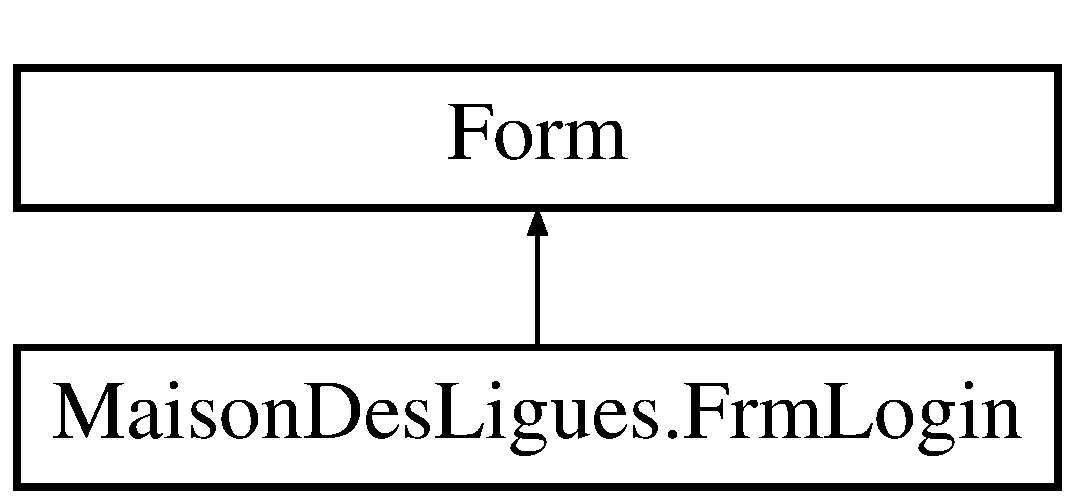
\includegraphics[height=2.000000cm]{class_maison_des_ligues_1_1_frm_login}
\end{center}
\end{figure}
\subsection*{Public Member Functions}
\begin{DoxyCompactItemize}
\item 
\hyperlink{class_maison_des_ligues_1_1_frm_login_a16d5a2efd1c29334f1a0ccf25c910b64}{Frm\+Login} ()
\begin{DoxyCompactList}\small\item\em constructeur \end{DoxyCompactList}\end{DoxyCompactItemize}
\subsection*{Protected Member Functions}
\begin{DoxyCompactItemize}
\item 
override void \hyperlink{class_maison_des_ligues_1_1_frm_login_a1b5a9829dc7217d8cca6c504b59cc9c6}{Dispose} (bool disposing)
\begin{DoxyCompactList}\small\item\em Nettoyage des ressources utilisées. \end{DoxyCompactList}\end{DoxyCompactItemize}


\subsection{Constructor \& Destructor Documentation}
\hypertarget{class_maison_des_ligues_1_1_frm_login_a16d5a2efd1c29334f1a0ccf25c910b64}{}\index{Maison\+Des\+Ligues\+::\+Frm\+Login@{Maison\+Des\+Ligues\+::\+Frm\+Login}!Frm\+Login@{Frm\+Login}}
\index{Frm\+Login@{Frm\+Login}!Maison\+Des\+Ligues\+::\+Frm\+Login@{Maison\+Des\+Ligues\+::\+Frm\+Login}}
\subsubsection[{Frm\+Login}]{\setlength{\rightskip}{0pt plus 5cm}Maison\+Des\+Ligues.\+Frm\+Login.\+Frm\+Login (
\begin{DoxyParamCaption}
{}
\end{DoxyParamCaption}
)}\label{class_maison_des_ligues_1_1_frm_login_a16d5a2efd1c29334f1a0ccf25c910b64}


constructeur 



\subsection{Member Function Documentation}
\hypertarget{class_maison_des_ligues_1_1_frm_login_a1b5a9829dc7217d8cca6c504b59cc9c6}{}\index{Maison\+Des\+Ligues\+::\+Frm\+Login@{Maison\+Des\+Ligues\+::\+Frm\+Login}!Dispose@{Dispose}}
\index{Dispose@{Dispose}!Maison\+Des\+Ligues\+::\+Frm\+Login@{Maison\+Des\+Ligues\+::\+Frm\+Login}}
\subsubsection[{Dispose}]{\setlength{\rightskip}{0pt plus 5cm}override void Maison\+Des\+Ligues.\+Frm\+Login.\+Dispose (
\begin{DoxyParamCaption}
\item[{bool}]{disposing}
\end{DoxyParamCaption}
)\hspace{0.3cm}{\ttfamily [protected]}}\label{class_maison_des_ligues_1_1_frm_login_a1b5a9829dc7217d8cca6c504b59cc9c6}


Nettoyage des ressources utilisées. 


\begin{DoxyParams}{Parameters}
{\em disposing} & true si les ressources managées doivent être supprimées ; sinon, false.\\
\hline
\end{DoxyParams}


The documentation for this class was generated from the following files\+:\begin{DoxyCompactItemize}
\item 
Maison\+Des\+Ligues/Frm\+Login.\+cs\item 
Maison\+Des\+Ligues/Frm\+Login.\+Designer.\+cs\end{DoxyCompactItemize}

\hypertarget{class_maison_des_ligues_1_1_frm_principale}{}\section{Maison\+Des\+Ligues.\+Frm\+Principale Class Reference}
\label{class_maison_des_ligues_1_1_frm_principale}\index{Maison\+Des\+Ligues.\+Frm\+Principale@{Maison\+Des\+Ligues.\+Frm\+Principale}}
Inheritance diagram for Maison\+Des\+Ligues.\+Frm\+Principale\+:\begin{figure}[H]
\begin{center}
\leavevmode
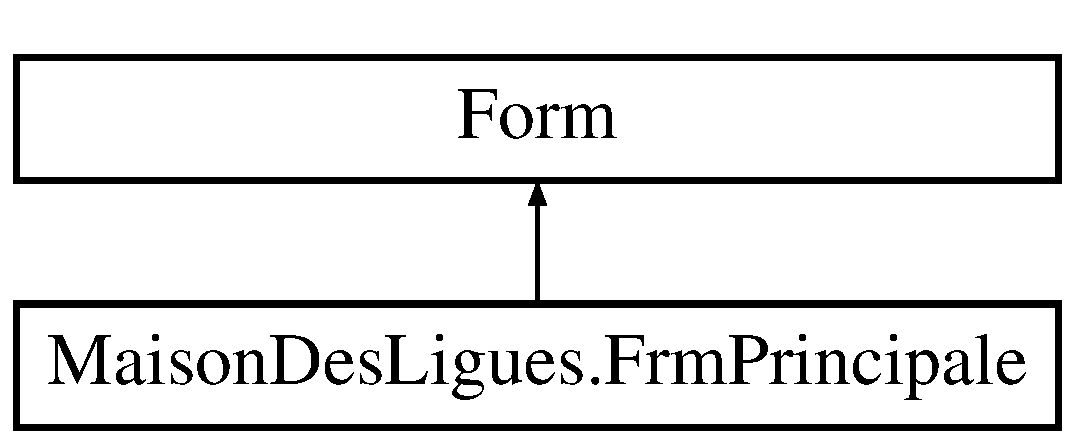
\includegraphics[height=2.000000cm]{class_maison_des_ligues_1_1_frm_principale}
\end{center}
\end{figure}
\subsection*{Public Member Functions}
\begin{DoxyCompactItemize}
\item 
\hyperlink{class_maison_des_ligues_1_1_frm_principale_a57b3b29fd74de6dba450eeddb60b0bce}{Frm\+Principale} ()
\begin{DoxyCompactList}\small\item\em constructeur du formulaire \end{DoxyCompactList}\end{DoxyCompactItemize}
\subsection*{Protected Member Functions}
\begin{DoxyCompactItemize}
\item 
override void \hyperlink{class_maison_des_ligues_1_1_frm_principale_a65be0e11ff6ef434dd448410efc60f00}{Dispose} (bool disposing)
\begin{DoxyCompactList}\small\item\em Clean up any resources being used. \end{DoxyCompactList}\item 
override void \hyperlink{class_maison_des_ligues_1_1_frm_principale_a65be0e11ff6ef434dd448410efc60f00}{Dispose} (bool disposing)
\begin{DoxyCompactList}\small\item\em Clean up any resources being used. \end{DoxyCompactList}\item 
override void \hyperlink{class_maison_des_ligues_1_1_frm_principale_a65be0e11ff6ef434dd448410efc60f00}{Dispose} (bool disposing)
\begin{DoxyCompactList}\small\item\em Clean up any resources being used. \end{DoxyCompactList}\item 
override void \hyperlink{class_maison_des_ligues_1_1_frm_principale_a65be0e11ff6ef434dd448410efc60f00}{Dispose} (bool disposing)
\begin{DoxyCompactList}\small\item\em Clean up any resources being used. \end{DoxyCompactList}\end{DoxyCompactItemize}


\subsection{Constructor \& Destructor Documentation}
\hypertarget{class_maison_des_ligues_1_1_frm_principale_a57b3b29fd74de6dba450eeddb60b0bce}{}\index{Maison\+Des\+Ligues\+::\+Frm\+Principale@{Maison\+Des\+Ligues\+::\+Frm\+Principale}!Frm\+Principale@{Frm\+Principale}}
\index{Frm\+Principale@{Frm\+Principale}!Maison\+Des\+Ligues\+::\+Frm\+Principale@{Maison\+Des\+Ligues\+::\+Frm\+Principale}}
\subsubsection[{Frm\+Principale}]{\setlength{\rightskip}{0pt plus 5cm}Maison\+Des\+Ligues.\+Frm\+Principale.\+Frm\+Principale (
\begin{DoxyParamCaption}
{}
\end{DoxyParamCaption}
)}\label{class_maison_des_ligues_1_1_frm_principale_a57b3b29fd74de6dba450eeddb60b0bce}


constructeur du formulaire 



\subsection{Member Function Documentation}
\hypertarget{class_maison_des_ligues_1_1_frm_principale_a65be0e11ff6ef434dd448410efc60f00}{}\index{Maison\+Des\+Ligues\+::\+Frm\+Principale@{Maison\+Des\+Ligues\+::\+Frm\+Principale}!Dispose@{Dispose}}
\index{Dispose@{Dispose}!Maison\+Des\+Ligues\+::\+Frm\+Principale@{Maison\+Des\+Ligues\+::\+Frm\+Principale}}
\subsubsection[{Dispose}]{\setlength{\rightskip}{0pt plus 5cm}override void Maison\+Des\+Ligues.\+Frm\+Principale.\+Dispose (
\begin{DoxyParamCaption}
\item[{bool}]{disposing}
\end{DoxyParamCaption}
)\hspace{0.3cm}{\ttfamily [protected]}}\label{class_maison_des_ligues_1_1_frm_principale_a65be0e11ff6ef434dd448410efc60f00}


Clean up any resources being used. 


\begin{DoxyParams}{Parameters}
{\em disposing} & true if managed resources should be disposed; otherwise, false.\\
\hline
\end{DoxyParams}
\hypertarget{class_maison_des_ligues_1_1_frm_principale_a65be0e11ff6ef434dd448410efc60f00}{}\index{Maison\+Des\+Ligues\+::\+Frm\+Principale@{Maison\+Des\+Ligues\+::\+Frm\+Principale}!Dispose@{Dispose}}
\index{Dispose@{Dispose}!Maison\+Des\+Ligues\+::\+Frm\+Principale@{Maison\+Des\+Ligues\+::\+Frm\+Principale}}
\subsubsection[{Dispose}]{\setlength{\rightskip}{0pt plus 5cm}override void Maison\+Des\+Ligues.\+Frm\+Principale.\+Dispose (
\begin{DoxyParamCaption}
\item[{bool}]{disposing}
\end{DoxyParamCaption}
)\hspace{0.3cm}{\ttfamily [protected]}}\label{class_maison_des_ligues_1_1_frm_principale_a65be0e11ff6ef434dd448410efc60f00}


Clean up any resources being used. 


\begin{DoxyParams}{Parameters}
{\em disposing} & true if managed resources should be disposed; otherwise, false.\\
\hline
\end{DoxyParams}
\hypertarget{class_maison_des_ligues_1_1_frm_principale_a65be0e11ff6ef434dd448410efc60f00}{}\index{Maison\+Des\+Ligues\+::\+Frm\+Principale@{Maison\+Des\+Ligues\+::\+Frm\+Principale}!Dispose@{Dispose}}
\index{Dispose@{Dispose}!Maison\+Des\+Ligues\+::\+Frm\+Principale@{Maison\+Des\+Ligues\+::\+Frm\+Principale}}
\subsubsection[{Dispose}]{\setlength{\rightskip}{0pt plus 5cm}override void Maison\+Des\+Ligues.\+Frm\+Principale.\+Dispose (
\begin{DoxyParamCaption}
\item[{bool}]{disposing}
\end{DoxyParamCaption}
)\hspace{0.3cm}{\ttfamily [protected]}}\label{class_maison_des_ligues_1_1_frm_principale_a65be0e11ff6ef434dd448410efc60f00}


Clean up any resources being used. 


\begin{DoxyParams}{Parameters}
{\em disposing} & true if managed resources should be disposed; otherwise, false.\\
\hline
\end{DoxyParams}
\hypertarget{class_maison_des_ligues_1_1_frm_principale_a65be0e11ff6ef434dd448410efc60f00}{}\index{Maison\+Des\+Ligues\+::\+Frm\+Principale@{Maison\+Des\+Ligues\+::\+Frm\+Principale}!Dispose@{Dispose}}
\index{Dispose@{Dispose}!Maison\+Des\+Ligues\+::\+Frm\+Principale@{Maison\+Des\+Ligues\+::\+Frm\+Principale}}
\subsubsection[{Dispose}]{\setlength{\rightskip}{0pt plus 5cm}override void Maison\+Des\+Ligues.\+Frm\+Principale.\+Dispose (
\begin{DoxyParamCaption}
\item[{bool}]{disposing}
\end{DoxyParamCaption}
)\hspace{0.3cm}{\ttfamily [protected]}}\label{class_maison_des_ligues_1_1_frm_principale_a65be0e11ff6ef434dd448410efc60f00}


Clean up any resources being used. 


\begin{DoxyParams}{Parameters}
{\em disposing} & true if managed resources should be disposed; otherwise, false.\\
\hline
\end{DoxyParams}


The documentation for this class was generated from the following files\+:\begin{DoxyCompactItemize}
\item 
Maison\+Des\+Ligues/Frm\+Principale.\+cs\item 
Maison\+Des\+Ligues/Frm\+Principale.\+Designer.\+cs\item 
Maison\+Des\+Ligues/Frm\+Principale.\+Designer.\+cs.\+B\+A\+S\+E.\+cs\item 
Maison\+Des\+Ligues/Frm\+Principale.\+Designer.\+cs.\+L\+O\+C\+A\+L.\+cs\item 
Maison\+Des\+Ligues/Frm\+Principale.\+Designer.\+cs.\+R\+E\+M\+O\+T\+E.\+cs\end{DoxyCompactItemize}

%--- End generated contents ---

% Index
\backmatter
\newpage
\phantomsection
\clearemptydoublepage
\addcontentsline{toc}{chapter}{Index}
\printindex

\end{document}
